\documentclass[twoside, a4paper, DIV=11,twocolumn]{book}
% \documentclass[oneside, a4paper, DIV=11]{book}

% PACKAGES
\usepackage[ngerman]{babel}
\usepackage[utf8]{inputenc}
\usepackage[singlespacing]{setspace} % 1,5 Zeilenabstand
%\usepackage{subscript} % Tiefegestellter Text außerhalb des Mathemodus
\usepackage{fixltx2e} % Tiefegestellter Text außerhalb des Mathemodus
\usepackage{amsmath,
	    amssymb,
	    array,
	    balance, % gleich lange säulen am ende jedes Kapitels
	    color,
	    graphicx,
	    hyphsubst, % Silbentrennung wie ich es will
	    hyperref,
	    natbib,
	    siunitx, 
	    tabularx,
	    tikz}

% \usepackage{pdflscape,}
%\hypersetup{linktocpage} % nur die Seitenzahlen erscheinen als Link
\usepackage{./src/mymacros}
\usepackage{./docu/bscmakros}


% \usepackage{showframe} % show margins and stuff

% SETTINGS

\hypersetup{
    colorlinks,
    citecolor=black,
    filecolor=black,
    linkcolor=black,
    urlcolor=black
}

\sisetup{
    locale=DE,
    loctolang={DE:ngerman},
    load-configurations = binary,
    binary-units = true,
    list-final-separator = { \translate{und} },
    list-units=single,
    range-phrase = { \translate{bis} },
    range-units=single,
    round-mode = places,
    round-precision = 3
}

%TITLE
\title{Transport durch Dichteinstabilitäten in einer Hele-Shaw Zelle}
\author{Johannes Haux}
\date{1.4.2015}

%DOCUMENT
\begin{document}

\onecolumn
\begin{titlepage}
\begin{center}
 
\Large\textbf{Department of Physics and Astronomy\\
University of Heidelberg}

\vspace{16cm}

\normalsize
Bachelor Thesis in Physics\\
submitted by \\
\vspace{0.5cm}
\Large\textbf{Johannes Stefan Jacob Haux}\\
\normalsize
\vspace{0.5cm}
born in Tübingen (Germany)\\
\vspace{0.5cm}
\Large\textbf{2015}
\normalsize

\newpage




\vspace{18cm}

\normalsize
This Bachelor Thesis has been carried out by Johannes Stefan Jacob Haux at the\\
Institute of Environmental Physics in Heidelberg\\
under the supervision of\\
Prof. Kurt Roth

\vfill
\end{center}

\end{titlepage}
 % von der Uni gefordert. ggf anpassen


% \maketitle
\chapter*{abstract}
 %Englisch
  
 %Deutsch
  In this work we will show the influence of densitiy driven instabilities and their 
\twocolumn
\tableofcontents
\listoffigures

\balance % gleich lange säulen am ende jedes Kapitels
\chapter{Einleitung}

% Gutes Verständis, da Bodenphysik immer gute Beisiele hat:
% Salzsee, CO2 einlagerung
\label{sec:intro}

Während der Durchführung meiner Bachelorarbeit entstanden zunächst Ideen zu einem Experiment, dass sich schließlich als nicht durchführbar herausstellte, für den zur 
Verfügung stehenden Zeitraum. In Folge dessen kam die Idee zu einem weiteren, für die zur Verfügung stehende Zeit besser geeignetem Experiment. Aus diesem Grund teilt
sich diese Arbeit in jedem ihrer Abschnitte immer in inhaltlich dem einen, wie dem anderen Experiment zugehörigen Bereiche.

Grundlegend für alle Fragestellungen, die im Laufe dieser Arbeit aufkamen, sind Dichteinstabilitäten, die zur treibenden Kraft von Prozessen werden, die mit Hilfe
einer Hele-Shaw-Zelle beobachtet werden sollen.
Zunächst wird die Frage gestellt, wie sich Verdunstungsphänomene auf Stofftransport in gesättigten, heterogenen, porösen Medien auswirken und zu Stofftransport 
von der Oberfläche in tiefere Schichten führt. Als Beispiel kann man sich einen Salzsee vorstellen, der dabei ist auszutrocknen und dabei Salz in tiefere Erdschichten
einlagert.
In einem zweiten Ansatz wird die Frage gestellt, wie sich in Wasser lösendes \COT für Dichteinstabilitäten sorgt, die schließlich das gelöste Gas in tiefer Wasserbereiche 
führt. Auch hier lässt sich wieder ein sehr Anwendungsbezogenes Beispiel finden, wie schon \cite{fernandez} treffend festgestellt hat: Das Einlagern von \COT in
Gesteinsschichten setzt vorraus, dass sich das \COT lange genug auf dem Gestein aufhält. Sorgt man dafür, dass unterirdische Wasserreservoirs mit \COT gesättigt werden
kann man dieses Verhalten künstlich herbeiführen. Ein Verständnis dafür, wie sich \COT in Wasser löst und bewegt ist dafür grundlegend.

Diese Arbeit ist gegliedert in folgende Teile: Zunächst soll in Teil \ref{sec:theo} eine theoretische Grundlage geschaffen werden, zum Verständis der folgenden Abschnitte.
Anschließend erkläre die Teile \ref{sec:set} "Experimenteller Aufbau" und \ref{sec:ima} "Bildanalyse" die Methoden, mit denen Messdaten beschaffen und ausgewerted wurden.
Die Ergebisse dieser Messungen werden in Teil \ref{sec:res} "Ergebnisse" präsentiert und diskutiert.
Am Ende folgt eine Zusammenfassunge mit Ausblick.

\chapter{Grundlagen}
\label{cha:theo}

Zur Beschreibung der beiden durchgeführten \HSCs-Experimente sind zwei Themengebiete von Interesse: Zum einen wird ein Ansatz benötigt um poröse Medien zu charakterisieren, zum anderen muss verstanden werden, wie das Ausbilden von Dichteinstabilitäten von statten geht und wie sich beispielsweise dadurch Finger bilden.

\section{Poröse Medien}
\label{sec:por}
Poröse Medien, wie beispielsweise Sand oder Ton, teilen den Raum, den sie füllen, in Matrix und Poren auf \citep{roth2005}.  Matrix bezeichnet in diesem Fall die Bereiche, an dem sich das feste Medium befinden, der eigentliche Sand. Die Poren bilden den zunächst leeren Raum dazwischen.
Als charakteristische Größen lassen sich die Porosität $\phi$ und die Raumdichte $\rho_{bulk}$ definieren:
\begin{align}
 \phi &= \frac{V_{pore}}{V_{tot}} \\
 \rho_{bulk} &= \frac{m_{matrix}}{V_{tot}} = \frac{\phi}{1-\phi}
\end{align}
$V_{pore}$ und $V_{tot}$ bezeichnen die Volumina, die von den Poren, bzw insgesamt eingenommen werden, $m_{matrix}$ die Masse der Matrix. 

\TODO{navier + leitfähigkeit}
\section{Hydraulik}
\label{sec:hyd}
Die Bewegung inkompressibler Fluidpartikel wird durch die Navier-Stoke Gleichung beschrieben:
\begin{eqnarray}
 \rho \dot{\vec{v}} = \rho \left( \frac{\partial \vec{v}}{\partial t} + \vec{v} \cdot \nabla \vec{v} \right) = - \nabla p + \mu \nabla^2 \vec{v} + \vec{f}
\end{eqnarray}
Hierbei bezeichnet $\vec{v}$ die Geschwindikeit des betrachteten Partikels, $\nabla p$ den Druckgradienten und $\mu \nabla^2 \vec{v}$ den Reibungsterm. $\vec{f}$ steht für äußere Kräfte, die auf das System wirken, wie zum Beispiel die Gravitationskraft. \citep{roth2005}



\TODO{solute transport}
\TODO{Konduktivität und Diffusivität => Reynolds}


\chapter{Experimenteller Aufbau}
\label{cha:set}

Da für beide in Teil \ref{cha:intro} beschriebenen Fragestellungen die Dynamik der betrachteten Systeme interessant ist, wird jeweils ein ``Light Transmission Experiment''
durchgeführt. Hierzu wird eine \HSC vor einer homogenen Lichtquelle platziert. Das Licht, dass die Zelle durchdringt wird von einer Digitalkamera aufgezeichnet und für die spätere Auswertung gespeichert.
Größter Unterschied bei den beiden durchgeführten Experimenten ist vor Allem die Dauer. Während das Verdunstungsexperiment fast zwei Wochen dauert ist das \COT-Experiment auf maximal wenige Stunden ausgelegt. 
\TODO{muss der letzte Satz sein? Gehört das hier hin?}
\widegraph[./plot/Aufb_Dunst.png]{Grundsätzlicher Aufbau der beiden durchgeführten Experimente. Zu sehen sind: 1: Lichtquelle, 2: \HSC, 3: Kamera}{fig:auf}

\subsection{\HSC}
\label{sec:hsc}
Der Vorteil einer \HSC ist, dass man mit Ihr Beobachtungen zweidimensionaler Natur machen kann.
Grundsätzlich besteht die Zelle aus zwei Glasplatten, die einem kleinen Abstand zueinander parallel angeordnet sind. Bei diesem Aufbau ist der Zwischenraum an drei der vier Seiten abgedichtet, sodass kein Wasser abfließen kann. Für Dichte wird gesorgt, indem die Glasplatten mit Hilfe von Keilen in einen Rahmen und gegen die Dichtgummis, welche auch als Abstandhalter dienen, gepresst werden. 
Die offene Seite der Zelle zeigt nach oben und am unteren Ende der Zelle befindet sich ein Ausfluss, über den die Zelle kontrolliert mit Wasser oder einer gewünschten Lösung befüllt werden kann.
Die Abmessungen der verwendeten Zellen sind in Tabelle \ref{tab:Hdim} festgehalten.


\inkscape{./plot/cell_dimensions.pdf_tex}{\linewidth}{Dimensionierung der \HSC. Ansicht von oben und von der Seite. 1:Keil, 2: Dichtung und Abstandhalter, 3: Rahmen, 4: Glasplatte, 5: Füllung der Zelle. \TODO{ersetzen der Maße durch Beschriftung}}{fig:Hdim}

\begin{table}[h]
  \begin{tabularx}{\linewidth}{X|c|c|c} %>{\raggedright}p{2,2cm}<{}
    Aufbau			& Höhe				& Breite			& Abstand \\
    \hline\hline
    Verdunstungs\-experi\-ment	& \SI{ 500}{\milli\meter}	& \SI{273}{\milli\meter}	& \SI{3}{\milli\meter} \\
    \hline
    \COT-			& \SI{ 250}{\milli\meter}	& \SI{273}{\milli\meter}	& \SI{2,1}{\milli\meter} \\
    Experiment			& \SI{ 500}{\milli\meter}	& \SI{273}{\milli\meter}	& \SI{2,1}{\milli\meter}
  \end{tabularx}
  \caption{Dimensionierung der \HSCs für die beiden durchgeführten Experimente. Siehe auch Abbildung \ref{fig:Hdim}.}
  \label{tab:Hdim}
\end{table}


\subsection{Kamera}
\label{sec:cam}
Die Messung wird mit Hilfe einer \TODO{AVT Pike F-505B}-Kamera durchgeführt. Diese wurde \TODO{erstmals} bei \cite{heberle} zum Einsatz gebracht und ausführlich beschrieben. 

Die Daten in \ref{tab:cam} sind aus dieser Arbeit sowie dem Internetauftritt des Herstellers \citep{pike_sheet} entnommen. 
\begin{table}[h]
 \begin{tabularx}{\linewidth}{X|c}
  Komponente	& Eigenschaft \\
  \hline\hline
  Kamera	& AVT Pike F-505B \\
  Sensortyp	& CCD \\
  Farbtiefe	& \SI{14}{bit}, monochrom \\
  Auflösung	& 2452 $\cdot$ 2054 Pixel \\
  Schnittstelle	& IEEE1394-B \\
  \hline
  Objektiv	& Fujinon HF50SA-1 \\
  Brennweite	& 50 mm \\
  \hline
  Filter 1	& \SI{452}{\nano\meter}, FWHM \SI{9}{\nano\meter} \\
  Filter 2	& \SI{632}{\nano\meter}, FWHM \SI{11}{\nano\meter} 
 \end{tabularx}
 \caption{Herstellerangaben zur verwendeten Kamera, sowie des Objektives und der Filter.}
 \label{tab:cam}
\end{table}
Die Kamera kann über die Firewire Schnittstelle gesteuert und ausgelesen werden. Auch das Auswählen des benötigten Filters kann mit Hilfe eines Filterrads vom Computer aus geschehen.

\subsection{Lichtquelle}
\label{sec:light}
Um eine möglichst gleichmäßige Durchleuchtung der Zelle zu bewerkstelligen wird ein Array aus LEDs der Farben Rot, Grün und Blau verwendet. Davor ist eine Diffusorfolie gespannt. Die Lichtquelle befindet sich zusätzlich in einem mit Alufolie ausgekleideten Kasten, in welchen auch Lüfter eingebaut sind. Per Computer lassen sich die LEDs zusammen mit der Lüftung ein und ausschalten. Auch hierzu finden sich wieder ausführliche Informationen bei \cite{buchner}\ und \cite{heberle}.


\section{Verdunstungsexperiment}
\label{sec:eva}

\graph{Aufbau des Verdunstungsexperiments. Zu Sehen sind 1. , 2. , ...}{gr:suevp}

Für den ersten Versuch wird ein bereits vorhandener Aufbau von \cite{feustel} gewählt, da die streng heterogenen Eigenschaften des aufgeschütteten porösen Mediums erwünscht sind. Hierbei ist die große \HSC ist mit Glaskügelchen verschiedener Größen gefüllt. Dabei wurde darauf geachtet, dass die immer homogene Regionen enstehen, die sich nicht komplett über die gesamte Zellbreite erstrecken, wie in Abbildung \ref{fig:het} zu sehen ist. 
Die Größen der verwendeten Kugeln (\textit{SiLi-Beads}) der Firma \textit{Sigmund-Lindner GmbH} sind in Tabelle \ref{tab:kug} notiert. 

\graph{Die heterogene Struktur des aufgeschütteten porösen Mediums. Die verschiedenen Bereiche unterschiedlicher Kugelgröße lassen sich mit Hilfe von Tabelle \ref{tab:kug} zuordnen.}{fig:het}
\begin{table}[h]
  \begin{tabularx}{\linewidth}{X|c|c|c}
		& Durch\-messer 			& Stdabw. d. \O{}			& Raumgewicht	\\
		& $\left[\si{\milli\meter}\right]$	& $\left[\si{\milli\meter}\right]$	& $\left[\si{\kg\per\dm\tothe{3}}\right]$ \\
    \hline\hline
    \circled{1}	& 0,07 - 0,11				& 0,06					& 1,37 \\
    \circled{2}	& 0,2 - 0,3				& 0,03					& 1,44 \\
    \circled{3}	& 0,4 - 0,6				& 0,21					& 1,47 
  \end{tabularx}
  \caption{Daten der verwendeten \textit{SiLi-Beads}. Die Materialdichte der Kugeln betragt \SI{2.5}{\kg\per\dm\tothe{3}}. Entnommen aus \cite{feustel}.}
  \label{tab:kug}
\end{table}

Für dieses Experiment wurde der Zufluss so eingerichtet, dass sowohl \COT als auch Wasser, bzw. gelöstes \BB kontrolliert in die Zelle geleitet werden können. \BB ist eine Nahrungsmittelfarbe, welche hier in einer Konzentration von \SI{0,05}{\gram\per\liter}. Er absorbiert im Wellenlängenbereich von \SI{630}{\nano\meter} maximal. Eine \BB Lösung kann also gut mit dem passenden Filter vor der Kamera verfolgt werden. Siehe auch hierzu Abbildung \ref{fig:het}.
Damit keine Luftblasen zwischen den Kügelchen zurückbleiben wird vor dem Fluten mit Wasser\COT durch die Zelle gespült. Dazu wir eine Flasche mit etwas Trockeneis befüllt und anschließend das entstehende Gas in die Zelle geleitet. Da gasförmiges \COT schwerer ist als Luft kann man es einfach laufen lassen. Nach etwas ein bis zwei Stunden wird angenommen, dass die gesamte Luft aus der Zelle verdrängt wurde und es wird Wasser zugeführt. In diesem löst sich das Gas, sodass das poröse Medium komplett mit Wasser gefüllt ist. Um unerwartete Efekte zu vermeiden wird anschließend noch länger Wasser durch die Zelle gepumpt, damit im Wasser, dass letztendlich in der Zelle ist, möglichst kein gelöstes \COT ist.
Zum Beginn des Experiments wird der Wasserspiegel auf Höhe der obersten Kugelschicht gesenkt und die Pumpschläuche entfernt.
Die Kamera filmt das Experiment mit einer Bildrate von \SI{1}{Bild\per\hour}. Ein Skript steuert die Beleuchtung, sodass diese kurz vor der Bildaufnahme angeht und kurz darauf wieder aus.



\section{\COT-Experiment}
\label{sec:cot}
Für das zweite Experiment wurde die \HSCs mit einer \BCG Lösung von \SI{3,5}{\milli\gram\per\liter} befüllt. 
\BCG ist eine Indikatorlösung, die von blau zu gelb umschlägt in einem pH-Bereich von 5,4 bis 3,9. Reines Wasser, dass nur mit Luft in Kontakt ist hat einen pH-Wert von 5,6, wohingegen Wasser in dem sich \COT gelöst hat einen pH-Wert von 3,9 annimmt. 
Der Farbumschlag des \BCG führt dazu, dass die zunächst fast neutrale Lösung nicht mehr stark im \SI{630}{\nano\meter}-Bereich absorbiert sondern bei \SI{450}{\nano\meter}. \TODO{Dieses Verhalten wird in Abbildung \ref{fig:bcg} deutlich gemacht.}

\graph{Absorbierende Eigenschaften von \BCG}{fig:bcg}
Diese Eigenschaft passt sehr gut zu den zur Verfügung stehenden Filtern und macht es möglich zu verfolgen wo \COT in Wasser gelöst ist.
Die Kamera filmt wieder das Experiment, dieses mal jedoch mit einer sehr viel höheren Bildrate von ca. \SI{1}{Bildern\per\minute}.  Es werden Aufnahmen mit dem \SI{630}{\nano\meter}- und dem \SI{450}{\nano\meter}-Filter gemacht, sowie Aufnahmen bei verschlossenem Objektiv, die später zur Dunkelstromkorrektur verwendet werden sollen. 
Mit Start des Experiments, frühestens jedoch nach der ersten Aufnahme, wird von oben \COT in die Zelle geleitet. Auch hier geschieht dies mit Hilfe von Trockeneis, dieses Mal allerdings wird das freigesetzte Gas bei niedriger Rate gepumpt. Damit sich in dem Behältnis für das Gas wirklich nur \COT befindet, ist dieses nach oben hin geöffnet, sodass die leichtere Luft verdrängt wird. Zwischen Lösung und oberer Kante der Glasplatten wurde ausreichend Platz gelassen, sodass sich eine breitere \COT-Schicht bilden kann.

\section{\COT Experiment im porösen Medium.}
\label{sec:cpm}
Als zusätzliche Fragestellungen war geplant die durch gelöstes \COT verursachten Dichteinstabilitäten auch in Kombination mit einem porösen Medium zu untersuchen. Dazu ist die Zelle wieder mit Glaskügelchen befüllt, ähnlich wie in Aufbau \ref{sec:eva}.
Die Durchführung ist ähnlich wie in \ref{sec:cot}. Beim Befüllen der Zelle wird allerdings darauf geachtet, dass diese sehr langsam befüllt wird um Lufteinschlüsse zu vermeiden. Ein vorheriges Spülen mit \COT ist nicht möglich, da das Exoieriment dadurch systematisch beeinflusst würde.
Als poröses Medium wurden neben den bekannten, in Teil \ref{sec:eva} benutzten Kügelchen auch neue, aus Borosilikatglas verwendet.
\TODO{Eigenschaften neue Kügelchen}



\chapter{Methoden}
\label{cha:met}

Alle durchgeführten Experimente wurden, wie in Kapitel \ref{cha:set} beschrieben, mit Hilfe einer Kamera aufgezeichnet. Die Auswertung beruht daher in einem 
ersten Schritt darin die gewünschten Informationen aus den Bildern zu gewinnen. In allen durchgeführten Experimenten ist dies die Verfolgung eines Tracers, 
welcher andere Absorptionseigenschaften hat, als das ihn umgebende Material.
In einem nächsten Schritt werden die so gewonnen Daten genommen und weiter ausgewertet, um Informationen über das Verhalten der Beobachteten Phänomene zu 
erhalten.

Im Folgenden werden häufig die Begriffe ``Helligkeit'', ``Grauwert'' und ``Intensität'' synonym verwendet. Sie bezeichnen alle die selbe Information: Den 
Grauwert \TODO{$i \geq 0$} eines Pixels, bzw. die Grauwerte eines Pixelarrays.

\section{Bildanalyse}
\label{sec:ima}
% verwendete Software
Die vorgenommenen Bildanalysen wurden mit Hilfe von \cite{python} (Version 2.7) durchgeführt. 
% Hauptsächlich wurden die Pakete OpenCV (Version 2, zum Laden der Bilder), numpy (Verarbeitung der Bilder, Matrixoperationen) und matplotlib (Darstellung/Speichern und Plotten) verwendet.
% Einlesen der Bilder
Ein Bild, welches von OpenCV eingelesen wird besteht aus drei \SI{8}{\bit} Kanälen. Da die Kamera aber ein monochromes Bild aufgezeichnet hat, ist davon 
auszugehen, dass das eigentlich einkanalige Bild künstlich auf drei Kanäle umgerechnet wurde. Der Einfachheit halber wird über die Kanäle gemittelt und man 
erhält ein Array aus Grauwerten mit dem weiter gerechnet wird.

% Differenzen Methode
Zur Bestimmung der Position eines Tracers stehen verschiedene Möglichkeiten zu Verfügung.
Unter der Annahme, dass die aufgezeichneten Bilder $\mathbf{B}$ zu allen Zeiten in allen Bereichen gleich belichtet sind, kann man ein Referenzbild $\mathbf{R}$ 
vom Rest der Bilder abziehen. Als Referenz wird das erste Bild der Messung, bei noch unverändertem Ausgangszustand gewählt.
Als Ergebnis erhält man Matrizen $\mathbf{C}$, welche in unveränderten Bereichen den Wert Null annehmen, ansonsten aber ungleich null sind:
\begin{eqnarray}
 \mathbf{C} = \mathbf{B} - \mathbf{R}
\end{eqnarray}


Allerdings lässt sich leicht feststellen, dass die aufgezeichneten Bilder in ihrer Helligkeit schwanken. Bilder die früher aufgezeichnet wurden sind heller, als 
solche, die später gemacht wurden. Um diesem Effekt entgegenzuwirken wird ein Algorithmus implementiert, der einen Bildbereich betrachtet, dessen Helligkeit 
während der gesamten Messung konstant bleiben sollte. Sei $\mathbf{B}$ ein beliebiges Bild der Messreihe und $\mathbf{R}$ das Referenzbild. Dann sind 
$\mathrm{M(\mathbf{B})}$ und $\mathrm{M(\mathbf{R})}$ die Arrays aus $N$ Pixeln, die den Bildbereich mit konstanter Intensität beschreiben. Aus allen Elementen 
wird der jeweilige Mittelwert dieser beiden Matrizen errechnet:
\begin{eqnarray}
 \mu_{\mathbf{B}} = \frac{1}{N} \sum_{i=1}^N \mathrm{M(\mathbf{B})}_i \\
 \mu_{\mathbf{R}} = \frac{1}{N} \sum_{i=1}^N \mathrm{M(\mathbf{R})}_i
\end{eqnarray}

Aus diesen Werten lässt sich nun ein Faktor $f$ zur Korrektur des Bildes errechnen, da gilt:
\begin{eqnarray}
 \mu_{\mathbf{R}} = f \cdot \mu_{\mathbf{B}}
\end{eqnarray}

Damit lassen sich alle Grauwerte des Bildes auf den passenden Wert korrigieren ($\mathbf{B}_{neu} = f \cdot \mathbf{B}$) und man erhält einen neuen Wert für die 
Differenzmatrix:
\begin{eqnarray}
 \mathbf{C} = f \cdot \mathbf{B} - \mathbf{R}
 \label{eq:norm}
\end{eqnarray}


% Quotientenmethode
Neben der schwankenden Helligkeit fällt auch noch auf, dass die LED-Beleuchtung zu einer Vignettierung der Aufnahme führt, da die Beleuchtung in der Mitte 
stärker als an den Rändern. Ein einfaches Substrahieren der Bilder führt also zu einer Unterschätzung der absoluten Grauwerte im Außenbereich, bzw. zu einer 
Überschätzung im Innenbereich des Bildes.
Unter der Annahme, dass diese Vignettierung über den Zeitraum der Messung konstant bleibt, wird anstelle der Subtraktion eine Division durchgeführt, \dah jedes 
Pixel $\mathbf{b}_{nm}$ des untersuchten Bildes wird durch das Pixel $\mathbf{r}_{nm}$ des Referenzbildes an selber Stelle geteilt, wobei gilt 
$\mathbf{B} = \mathbf{b}_{nm}$ und $\mathbf{R} = \mathbf{r}_{nm}$. Zusammen mit Gleichung \ref{eq:norm} erhält man folgende Bildungsvorschrift für die 
Quotientenbilder:
\begin{eqnarray}
 \mathbf{C} = \mathbf{c}_{nm} = \frac{f * \mathbf{b}_{nm}}{\mathbf{r}_{nm}}
 \label{eq:quot}
\end{eqnarray}
Die Werte von $\mathbf{C}$ nehmen den Wert 1 überall dort an, wo Referenz- und betrachtetes Bild gleich sind. Der Tracer befindet sich also dort, wo gilt 
$\mathbf{c}_{nm} \neq 1$.

Zur leichteren Interpretation werden die Werte vor der graphischen Visualisierung auf einen Wertebereich von 0 bis 100 normiert.

\section{Detektion und Verfolgung des Tracers im Fall von Fingerbildung}
\label{sec:track}
Während der \COT-Experimente wird beobachtet, dass sich herabsinkende Finger der Wasser-\COT-Lösung, bilden. Deren Position und Länge über den Zeitraum der 
Messung, bzw. der ersten Minuten, sind interessante Größen, die dabei helfen können, das System zu beschreiben und zu verstehen.

Wird im folgenden von ``Bild'' gesprochen, so ist vom Quotientenbild nach Gleichung \ref{eq:quot} die Rede. Mit anderen Worten bezeichnet ``Bild'' die räumlich 
aufgelöste Tracerkonzentration zu einem bestimmten Zeitpunkt der Messung.

\subsection{Detektion}
\label{sec:dec}
Zunächst wird ein Bereich des zu untersuchenden Bildes festgelegt, in dem sich nur Indikatorflüssigkeit befindet. Nach Möglichkeit schließt die obere Kante 
dieses Bildbereiches genau mit der Wasserkante ab. Ein Herausragen über die Wasserkante wird vermieden, da die Hintergrundbeleuchtung für sehr helle 
Intensitätswerte sorgt. Da auch die Finger für höhere Intensitäten sorgen (siehe Teil \ref{sec:cot}) würde sonst die Messung systematisch beeinflusst. Der 
Bereich bleibt für alle Bilder gleich.

Aus dem so erhaltenen Array $\mathbf{C} = \mathbf{c}_{nm}$ ($n \in 1,\dots,N$ und $m \in 1,\dots,M$) wird von jeder Säule der Mittelwert berechnet. Man erhält 
ein Array der mittleren, vertikalen Intensitäten $\mathbf{I} = \mathbf{i}_{n}$:
\begin{eqnarray}
 \mathbf{i}_{n} = \frac{1}{M} \sum_{i=1}^{M} \mathbf{c}_{ni}
\end{eqnarray}

Für jedes Bild, bzw. jeden Zeitschritt erhält man so ein charakteristisches Signal. Unter der Annahme, dass die Finger sich gerade nach unten bewegen, befindet 
sich ein Finger an jedem lokalen Maximum von $\mathbf{I}$. Über die Richtigkeit dieser Annahme wird in Teil \ref{res:cot} diskutiert.
Da das Signal verrauscht ist wird eine diskrete Fourieranalyse durchgeführt, um das Wellenzahlenspektrum zu erhalten. So kann analysiert werden, in welchen 
Abständen Finger vorwiegend auftreten. Bereinigt man dieses Spektrum von den Werten, die dem Rauschen zugeordnet werden und führt eine Rücktransformation in den 
ursprünglichen Raum durch, kann man genau sehen, wo sich die Intensitäts-Maxima befinden. Wiederholt man dieses Verfahren zu jedem Zeitschritt erhält man eine 
zeitaufgelöste Vorstellung davon, wo sich die Finger im Verlauf des Experiments befinden.

\subsection{Länge}
\label{sec:lan}
Mit dem Wissen, wo sich die Finger befinden, lässt sich auch deren Länge errechnen. Dazu wird an jeder Stelle $s$ im Array $\mathbf{C}$ aus Teil \ref{sec:dec}, 
wo sich ein Finger befindet, die Pixelsäule $\mathbf{c}_{sm}$ von unten nach oben abgewandert ($m \in M, \dots, 1$), bis ein Schwellenwert $c_{crit}$ 
überschritten ist, der festlegt, ab welchem Grauwert von einem Finger die Rede ist. Um dieses Wert nicht durch Rauschen zu früh zu detektieren, wird über eine 
Reihe von 5 Pixeln links und rechts von $\mathbf{c}_{sm}$ gemittelt. Der so erhaltene Wert für $m(c_{crit})$ gibt die Länge $l$ des Fingers in Pixeln an.
\begin{align}
 m &\in (M,\dots,1) \\
 l(m) &= \left(\frac{1}{10}\sum_{i=s-5}^{s+5} \mathbf{c}_{im} \leq c_{crit} \right) \, ? \; l(m-1) : m \\
 l(0) &= 0
\end{align}

In Abbildung \ref{fig:four} und \ref{fig:len} sind Beispiele für die Detektion und bestimmte Länge der Finger zu finden.

\subsection{Wachstum}
\label{sec:grow}
Mit der Annahme, dass alle Finger gleich schnell wachsen, reicht es aus, zu jedem Zeitschritt $t_i$ den Mittelwert $\bar{l}_i$ der Länge aller Finger zu 
berechnen und anschließend durch den Zeitschritt zu teilen, um ihre Wachstumsrate zu ermitteln. 
\begin{align}
 \dot{l}_i &= \frac{\bar{l}_i-\bar{l}_{i-1}}{t_i-t_{i-1}} \\
 i &\in \mathbb{N} \\
 \bar{l}_{0} &= 0
\end{align}
man aber beobachten kann, dass die Finger in unterschiedlichen Bereichen unterschiedlich schnell wachsen, wird eine Methode implementiert, die es erlaubt, Teile 
des untersuchten Arrays $\mathbf{C}$ zu betrachten. Das bedeutet, es werden nur die Längen der Finger in diesem Bereich in Betracht gezogen. \TODO{Wählt man den 
Bereich klein genug ist es möglich auch einzelne Finger zu betrachten. ACHTUNG! wurde noch nicht gemacht}

\chapter{Ergebnisse}

\label{cha:res}
% \section{Verdunstungsexperiment}
% \label{res:eva}
% 
% \subsection{Präsentation}
% \label{res:eva:pres}
% 
% \widegraph[./plot/plot_eva]{Das Verdunstungsexperiment (a) zu Beginn der Messung und (b) am Ende nach 16 Tagen und 1,5 Stunden. Die Aufnahmen enstanden in Kombination mit einem \SI{630}{\nano\meter}-Filter. Die Ausbreitung den \BB Tracers ist mit einer weißen gestrichelten Linie bei (b) und (c) eingezeichnet. (c) Zeigt die Differenz der beiden Bilder (siehe Teil \ref{sec:ima}), normiert auf den Wertebereich $(0,\dots,100)$. Man kann erkennen, dass die Zelle im Verlauf der Messung gekippt ist (rote und blaue Streifen im oberen Teil des Bildes).}{fig:reseva}
% 
% 
% Das Verdunstungsexperiment wurde über einen Zeitraum von 16 Tagen und 1,5 Stunden durchgeführt. In Abbildung \ref{fig:reseva} kann man das Ergebnis der Messung sehen. Klar zu erkennen ist, dass sich der \BB-Tracer weit nach oben ausgebreitet hat, ca. über die Hälfte der Zelle. Bevorzugt wurde dabei der Weg über die Mitte der Zelle, was an der keilartigen struktur der Tracerausbreitung ausgemacht wird. 
% 
% Mit Hilfe der Differenzenmethode aus Teil \ref{sec:ima} und durch betrachten der Abfolge aller aufgenommener Bilder in Form eines Films, lässt sich erkennen, dass die Zelle über den Zeitraum des Experiments leicht nach vorne gekippt ist. Dadurch bilden sich rote und blaue Linien aus, da die flaschen Regieonen voneinander abgezogen werden. Eine Abschätzung, wie der Tracer sich ausgebreitet hat ist dennoch in Kombination mit der Originalaufnahme sehr gut möglich und reicht für die qualitative Abschätzung, wie sie hier erfolgen soll.
% 
% 
% \subsection{Schlussfolgerungen}
% \label{res:eva:disk}
% 
% Eine sehr grobe Abschätzung der Menge, des verdunsteten Wassers kann über die Fläche, die der Tracer einnimmt gemacht werden. So wie sie hier durchgeführt wird, kann und soll sie keine harten wissenschaftlichen Daten liefern, aber in Zahlen fassen, was man intuitiv sieht.
% 
% Unter der Annahme, dass die Kügelchen in der Zelle so dicht wie möglich gepackt sind ist die Porosität an allen Stellen $\bar{\phi} = 0,35$. Diese Annahme stellt natürlich eine untere Grenze dar, da die Kugeln nicht perfekt liegen. 
% Die eingenommene Fläche wird mit $\frac{1}{3}$ der Zellenfläche abgeschätzt. Zusammen mit den Abmessungen der Zelle (Tabelle \ref{tab:hsc}) erhält man das abgeschätzte Volumen $V_w$ des verdunsteten Wassers:
% \begin{align}
%  V_{HS-Zelle} &=  \SI{0,4095}{\liter} \\
%  \Rightarrow V_{w} &= \frac{\bar{\phi}}{3} \cdot V_{HS-Zelle} = \SI{0,04778}{\liter}
% \end{align}
% Teilt man dieses Ergebnis durch die Zeitdauer des Experiments erhält man eine Abschätzung für die Verdunstungsrate:
% \begin{align}
%  \dot{V_w} = \SI{0.1239}{\milli\liter\per\hour}
% \end{align}
% 
% \TODO{Vergleich Arbeit Apple}



% \newpage
\section{\COTm Experiment}
\label{res:cot}

\graph[./plot/plots_data-1/cell_patches]{Foto des Aufbaus. Mit roten Rechtecken sind die Bereiche zur Stabilisierung der Helligkeit (oben rechts) und zur tatsächlichen Auswertung (unten) markiert. Von oben kommt der Schlauch, durch welchen das \COT zugeführt wird ins Bild.}{fig:fotoau}

Wie in Teil \ref{cha:set} beschrieben wurde das \COTm Experiment mit der kleinen \HSC durchgeführt. Ein Foto des Aufbaus ist in Abbildung \ref{fig:fotoau} zu sehen. Dort sind auch der Bereich zur Stabilisierung der Helligkeit und der für die Messungen analysierte Bereich eingezeichnet.

Zunächst werden im folgenden Abschnit die gemachten Beobachtungen geschildert, anschließend werden sie interpretiert und diskutiert.


\subsection{Beobachtungen}
\label{res:cot:beob}

\sisetup{
  round-mode=places,
  round-precision=1
}


% ========================= Allgemeiner Verlauf =========================
In den Abbildungen \ref{fig:fft} bis \ref{fig:difkon} und \ref{fig:vcot_1-1} \ref{fig:complete} sind die Ergebnisse des \COTm Experiments festgehalten. Die Gesamtdauer des Experiments beläuft sich auf \mbox{\SI{5}{\hour} \SI{6}{\minute}}, der für diese Arbeit interessante Übergang zur Fingerbildung findet nach \SI{9}{\minute} statt. Nach ca. \SI{1,5}{\hour} wird das Verhalten zunehmend von Vortizitäten, die die ganze Zelle erfassen dominiert, weshalb spätestens hier alle in Teil \ref{cha:meth} beschriebenen Methoden versagen. 
Die Vortizitäten auf Zellskala sorgen für Durchmischung, da durch sie die Finger nicht mehr gerade nach unten sinken können, sondern zur Seite driften.

Wie erwartet kann die Fingerbildung beobachtet werden. Abbildungen \ref{fig:vcot_1-1}, \ref{fig:vcot_1-2} und \ref{fig:vcot_1-grey} zeigen ihren zeitlichen Verlauf.


% ========================= fft & k_space =========================
\widegraph[./plot/plots_data-1/fft]{Die mit Hilfe der diskreten Fourieranalyse vom Rauschen bereinigten mittleren Intensitäten der Finger. Der zeitliche Verlauf ist farblich codiert und geht von \SI{0}{\minute} (hellblau) bis \mbox{\SI{1}{\hour} \SI{24}{\minute}} (pink).}{fig:fft}

\graph[./plot/plots_data-1/k_space]{Mit Hilfe der diskreten Fourieranalyse bestimmtes Spektrum der Wellenzahlen. Man kann gut erkennen, dass $k \approx \SI[round-precision=2]{0,66}{\per\centi\meter}$ die dominierende Wellenzahl ist. Der zeitliche Verlauf ist farblich codiert und geht von \SI{0}{\minute} (hellblau) bis \mbox{\SI{1}{\hour} \SI{24}{\minute}} (pink).}{fig:k_space}

Zur Fingerdetektion wurde, wie in Teil Teil \ref{sec:dec} beschrieben, eine Fourieranalyse der mittleren Fingerintensitäten durchgeführt. Die resultierenden Spektren der Wellenzahlen $k(t)$ sind in Abbildung \ref{fig:k_space} zu sehen. Hier kann man erkennen, dass über den ersten Zeitbereich des Experiments zwischen 9 und \SI{60}{\minute}, ein Abstand von \SI[round-precision=2]{1,517}{\centi\meter} (entspricht $k=\SI[round-precision=2]{0,66}{\per\centi\meter}$) zwischen den Fingern dominiert und im zeitlichen Verlauf stabil bleibt. 

Die mit Hilfe dieser Fourieranalyse bereinigten mittleren Fingerintensitäten ist in Abbildung \ref{fig:fft} dargestellt. Ihr zeitlicher Verlauf ist farblich kodiert. Es wurden alle Signale mit einer Wellenzahl $k > \SI{2}{\per\centi\meter}$ als Rauschen eingestuft und ausgefiltert. Hier kann man gut das Wachstum der Finger in Form der steigenden Amplitude, sowie die Bewegung der Finger, erkennen. %, die relativ konstant bleibt. 

% ========================= Fingerzahl =========================
% \graph[./plot/plots_data-1/fcount]{Anzahl der detektierten Finger im Verlauf des Experiments. Das Rauschen tritt auf, da die Methode nicht einwandfrei funktioniert. Siehe dazu auch \ref{fig:f_detect}. Im Zeitraum von \SIrange{9}{40}{\minute} liefert sie allerdings relativ verlässliche Ergebnisse.}{fig:fcount}

\graph[./plot/plots_data-1/fgrowth]{Länge der detektierten Finger im Verlauf des Experiments. Das Rauschen tritt auf, da die Methode nicht einwandfrei funktioniert. Siehe dazu auch Abbildung \ref{fig:f_detect}. Im Zeitraum zwischen \SIrange{9}{40}{\minute} liefert sie zuverlässige Ergebnisse.}{fig:fgrowth}

% Die Graphen \ref{fig:fcount} und \ref{fig:fgrowth} zeigen Zahl und mittlere Länge der Finger über den Verlauf der Messung. 
Graph \ref{fig:fgrowth} zeigt die mittlere Länge der Finger im Verlauf der Messung. Für diese Betrachtung wurde der untersuchte Bereich der \HSC in 9 gleich große Teile aufgeteilt und über die Längen der Finger in diesen Bereichen gemittelt, um zu sehen, ob das Wachstum in verschiedenen Bereichen der Zelle unterschiedlich ist. 
Hier zeigt sich, was auch in Abbildung \ref{fig:vcot_1-1} zu erkennen ist: die Länge der Finger nimmt linear im Lauf der Zeit zu, mit gleicher Rate in allen Bereichen.

% einzelner Finger
Für generauere Betrachtung des Übergangs vom diffusiven zum konvektiven Vermischungsprozess von Wasser und \COT sind in Abbildung \ref{fig:vcot_1-grey} und \ref{fig:sevo} die ersten \SI{16}{\minute}, beziehungsweise \SI{52}{\minute} des Experiments gezeigt. Hierfür wurden die originalen Aufnahmen verwendet, da man hier deutlicher den Effekt beobachten kann.

Man kann erkennen, dass im Verlauf des Experiments, von \SI{5}{\minute} zu \SI{9}{\minute} der Übergang stattfindet. Anschließend bilden sich Finger aus. Direkt zu Beginn der Fingerbildung kann man sehen, wie die diffusive Schicht abgesaugt wird, ebenso wie kürzere Finger. Dies wird in Abbildung \ref{fig:sevo} (\SIrange{9}{26}{\minute}) besonders deutlich. In diesem Zeitraum kann man beobachten, wie rechts und links von dem am größten hervorragenden Finger die diffusive Schicht kleiner wird, bis fast wieder reines Wasser an der Wasseroberfläche ist. Nach \SI{24}{\minute} ist die obere \COT Schicht wieder so dick wie nach \SI{9}{\minute}. Nach \SI{39}{\minute} sorgen Vortizitäten dafür, dass die Schicht wieder dünner und vom Finger abgeführt wird.

Letztendlich verschmelzen nach einer Stunde immer mehr Finger miteinander (siehe \zB Abbildung \ref{fig:complete}). Diese wandern entlang der Wasseroberfläche.
Nach \SI{5}{\hour} ist die Zelle gut, wenn auch noch nicht komplett, durchmischt.


\subsection{Diskussion}
\label{res:cot:disk}

Ein Vergleich der oben gezeigten Ergebnisse mit denen aus anderen Arbeiten zeigen gute Übereinstimmungen.
\cite{kneafsy} beschreiben in Ihrer Arbeit sehr ähnliche Phänomene beim Lösen von \COT in Wasser in einer \HSC, so wie sie auch hier zu beobachten sind. Auch dort wird der Effekt beobachtet, dass die diffusive Schicht, welche sich zunächst ausbildet, mit Entstehen der Finger dünner wird.

Grund für dieses Verhalten ist die Konvektion des \COTm haltigen Wassers (siehe Abbildung \ref{fig:difkon}). 
% Durch die Abwärtsbewegung dieser dichteren Lösung, wird klares Wasser von unten nach oben transportiert. Dieses kann nun wieder leichter \COT aufnehmen, im Vergleich zum Wasser, in dem sich bereits \COT gelöst hat und damit ggf. schon gesättigt ist.

Was beobachtet werden kann sind zwei Prozesse, die einander beeinflussen: 
\begin{itemize}
 \item Mittels Diffusion wird das gelöste \COT langsam in tiefere Wasserschichten gebracht.
 \item Sobald die dadurch ausgebildete Schicht instabil wird, brechen Finger hervor. Es beginnt ein konvektiver Prozess, der das gelöste \COT schneller in noch tieferes Wasser bringt.
 \item Dadurch wiederum gelangt reines Wasser an die Oberfläche, was wiederum die Lösung von \COT im Wasser begünstigt.
 \item Neues \COT wird im Wasser gelöst und über die Konvektionskanäle, also die Finger, abtransportiert.
\end{itemize}

Abbildung \ref{fig:difkon} veranschaulicht das Beschriebene.
 
Die stabilen Abstände zwischen den Fingern, in den ersten \SI{60}{\minute}, lassen sich auch durch die konvektiven Prozesse zu Beginn erklären. Diese wirken stabilisierend auf die Finger, solange keine Vortizitäten auf Zellskala auftreten.
Intuitiv macht es Sinn, dass die Abstände der Finger in Größenordnung ihrer Breite sein sollte, da das durch die Finger verdrängte Volumen dem nach oben gedrängten entsprechen muss. Dieses Verhalten wird beobachtet.
Ähnliche Beobachtungen zur Stabilisierung der Fingersabstände werden von \cite{fernandez} gemacht. Auch dort dominiert ein Abstand zu Beginn der Fingerbildung. 

Das Verhalten der Finger, das nach spätestens \SI{60}{\minute} zu beobachten ist, lässt sich ähnlich erklären. Da die Zelle endlich tief ist, entstehen durch die Abwärtsbewegung des gelösten \COT Vortizitäten in Größenordnung der Zellentiefe. Diese führt dazu, dass die Finger nach außen driften und die Zelle nach und nach durchmischt wird.

Damit lässt sich das Experiment insgesamt in drei Phasen gliedern:
\begin{itemize}
 \item Diffusion (\SI{0}{\minute} bis \SI{9}{\minute})
 \item stabile Fingerbildung (\SI{9}{\minute} bis \SI{60}{\minute})
 \item Vortizitäten auf Zellebene (\SI{60}{\minute} bis zum Ende) 
\end{itemize}


Bei der Auswertung dieser Messung gibt es mehrere bekannte Fehlerquellen, die an dieser Stelle Erwähnung finden sollen. Zum einen sind die Aufnahmen, aufgrund der niedrigen Belichtungszeit verrauscht, was die Fingerdetektion und -längenmessung, trotz Stabilisierung der Bildhelligkeit, fehleranfällig macht.

Ein weitaus größeres Problem ist allerdings das Schwanken der Belichtung der Kamera. Leider konnte nicht herausgefunden werden, woher dieser Effekt kommt. Was man feststellen kann ist, dass die Kamera im Laufe der Zeit immer dunklere Bilder macht. Dieser Effekt sollte, durch die in Teil \ref{sec:ima} beschriebene Methode zur Korrektur der Helligkeitsschwankungen ausgeglichen werden. Leider konnte die angewandte Methode allerdings, nicht die gewünschten Ergebnisse liefern. Die Helligkeit der Bilder schwankt trotz allem im analysierten Bereich, wenn auch weniger stark. Dennoch führt dies dazu, dass, wie man in Abbildung \ref{fig:vcot_1-1} sehen kann, die Intensitäten der Finger schwanken und schwächer werden. Auch das führt zu fehlerhaften Längenbestimmungen der Finger, da der Grenzwert (siehe Teil \ref{sec:lan}) zu spät erreicht wird.

Diese Fehlerquellen wirken sich aber nicht negativ auf die Bestimmung der Fingerabstände über die Fourieranalyse aus, da die mittleren Intensitäten, trotzdem das charakteristische Wellenmuster (siehe Abbildung \ref{fig:fft}) aufweisen. Die Werte, welche aus diesen Messungen gewonnen wurden sind somit aussagekräftig.

\graph[./plot/Konvektion_Diffusion.pdf]{Interpretation der auftretenden Phänomene, verursacht durch Konvektion und Diffusion. Durch das Absinken der Finger wird Wasser mit gelöstem \COT aus der diffusiven Schicht, direkt unter Wasseroberfläche, abtransportiert und klares Wasser nach oben gedrückt. Dadurch kann sich wiederum mehr \COT im Wasser lösen.}{fig:difkon}


% \onecolumn
% 
% \begin{figure}
%  \centering
%  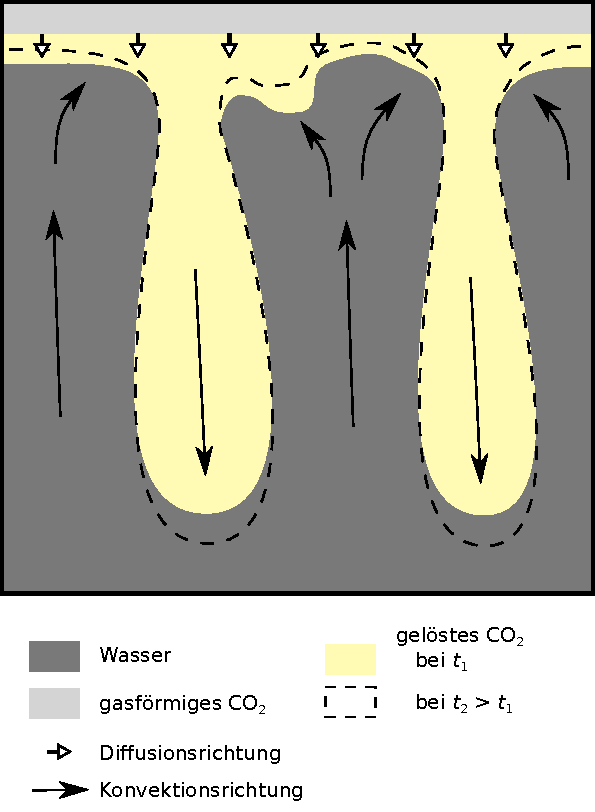
\includegraphics[width=9cm]{./plot/Konvektion_Diffusion.pdf}
%  \caption{Interpretation der auftretenden Phänomene, verursacht durch Konvektion und Diffusion}
%  \label{fig:difkon}
% \end{figure}
% 
% \twocolumn


% \newpage
% \mbox{\,}
\newpage

\section{\COTm Experiment mit porösem Medium}
\label{res:cpm}

\graph[./plot/BCG_test_03_num]{Farbumschläge des \BCG in Verbindung mit verschiedenen Substanzen. \BCG (1) in neutraler Form, \dah im Gleichgewicht mit der umgebenden Luft, (2) in Kombination mit \COT, (3) mit den Glaskügelchen verschiedener Größen, (4) mit Glaskügelchen und gelöstem \COT.}{fig:CPO}

\graph[./plot/BCG_Test_Boro_num]{Farbumschläge des \BCGn. \BCG (1) in neutraler Form, \dah im Gleichgewicht mit der umgebenden Luft, (2) in Kombination mit gelöstem \COT, (3) mit den Glaskügelchen aus \BOG, (4) mit Glaskügelchen und gelöstem \COTn.}{fig:CPO_bor}

Der Versuch das \COTm Experiment in einer mit einem porösen Medium gefüllten \HSC durchzuführen ist aufgrund der verwendeten Glaskugeln gescheitert. Glas macht Wasser durch Ionenaustausch basisch. Die leicht löslichen Elemente an der Oberfläche des Glases werden vom Wasser herausgelöst und durch die im Wasser vorhandenen H$^+$-Ionen ersetzt. Dadurch wird das Wasser basisch, da die OH$^-$-Konzentration steigt \citep{Vogel}.

Dieser Effekt ist durch die große Oberfläche, die die Kügelchen insgesamt haben, nicht zu vernachlässigen und sorgt dafür, dass der benutze Indikator nur den basischen Farbton annimmt. Das Lösen von \COT im Wasser kann diesen Effekt offensichtlich nicht überwiegen.

Zur Verdeutlichung der beschriebenen Phänomene siehe Abbildung \ref{fig:CPO}. Man kann erkennen, dass der Indikator einwandfrei das gelöste \COT anzeigt, solange sich nicht zusätzlich Kügelchen dabei sind. In diesem Fall bleibt der Indikator blau, auch wenn \COT im Wasser gelöst ist.

Ein angedachter Lösungsansatz mit Glaskugeln, welche dem Wasser gegenüber beständiger sind, konnte aus Zeitgründen nicht umgesetzt werden. Wie man in Abbildung \ref{fig:CPO_bor} sehen kann ergab ein Test der Kugeln aus Borosilikatglas aber vielversprechende Ergebnisse, da der durch das \COT hervorgerufene Farbumschlag auch mit Kugeln in der Indikatorlösung beobachtet werden konnte.

% \vspace{10cm} % damit balance die Bilder beide auf die Seite packt



  
% ========================= longgraphpages =========================
\longgraphpage[./plot/plots_data-1/plot_all_overview_quot_0]{(1/2) Fingerbildung im \COTm Experiment. Die Farbskala beschreibt die relative Absorption im Bezug auf den Hintergrund. Maximale Absorption bekommt den Wert 100 zugewiesen, minimale 0.}{fig:vcot_1-1}
\longgraphpage[./plot/plots_data-1/plot_all_overview_quot_1]{(2/2) Fingerbildung im \COTm Experiment. Die Farbskala beschreibt die relative Absorption im Bezug auf den Hintergrund. Maximale Absorption bekommt den Wert 100 zugewiesen, minimale 0.}{fig:vcot_1-2}

\longgraphpage[./plot/plots_data-1/finger_detection_cut]{Abgebildet sind die Fingerbildung zusammen mit den detektierten Fingerpositionen und -längen zur Demonstration, wie die in Teil \ref{sec:lan} beschriebene Methode funktioniert. Die Farbskala beschreibt die relative Absorption im Bezug auf den Hintergrund. Maximale Absorption bekommt den Wert 100 zugewiesen, minimale 0.}{fig:f_detect}


\longgraphpage[./plot/plots_data-1/plot_all_overview_0_adj]{Fingerbildung im \COTm Experiment. Rohaufnahmen mit erhöhtem Kontrast. Zu erkennen ist der Übergang vom diffusiven zum konvektiven Prozess bei ca. \SI{9}{\minute}. Auch kann man beobachten, wie die diffusive Schicht zwischen den Fingern ``abgesaugt'' wird. }{fig:vcot_1-grey}
% ========================= einzelner Finger =========================
\longgraphpagetriple{./plot/plots_data-1/single_evolution_1}{./plot/plots_data-1/single_evolution_2}{./plot/plots_data-1/single_evolution_3}{Entwicklung eines einzelnen Fingers mit der Zeit. Rohaufnahmen mit erhöhtem Kontrast. Zu erkennen ist der Übergang vom diffusiven zum konvektiven Prozess bei ca. \SI{9}{\minute}, sowie das Dünner werden der diffusiven Schicht rechts und links vom Finger im Zeitraum zwischen \SI{9}{\minute} und \SI{24}{\minute}}{fig:sevo}

\longgraphpagesextuple{./plot/plots_data-1/comp_evolution_1}{./plot/plots_data-1/comp_evolution_2}{./plot/plots_data-1/comp_evolution_3}{./plot/plots_data-1/comp_evolution_4}{./plot/plots_data-1/comp_evolution_5}{./plot/plots_data-1/comp_evolution_6}{Überblick über den gesamten Verlauf des Experiments. Zu Erkennen sind die beiden letzten Phasen in die sich der Verlauf des Experiments gliedert: stabile Fingerbildung und die ausbildung von Vortizitäten, die für Durhcmischung der Zelle sorgen. Die Phase, in der sich die diffusive Schicht ausbildet ist zu kurz, als dass sie bei dieser Zeitauflösung zu erkennen wäre. Sie kann in Abbildung \ref{fig:vcot_1-grey} betrachtet werden.}{fig:complete}
% \widegraphpage[./plot/plots_data-1/fingers_quot-raw_5-30_cut.png]{Vergleich der Quotientenmethode und dem tatsächlich aufgezeichneten Bild.}{fig:fing_comp}


% \chapter{Ausblick}
% \input{./docu/06_Schlussfolgerungen}

\chapter{Zusammenfassung}

\label{cha:con}

In dieser Arbeit wurde gezeigt, wie sich durch das Lösen von \COT in Wasser Dichteinstabilitäten ausbilden, welche zu Fingerbildung und damit \COTm Sequestration führen. 
Hierzu wurden Experimente in einer \HSC durchgeführt, welche für eine quasi zweidimensionale Versuchsanordnung sorgt. Mittels eines Indikators wurde die Ausbreitung des \COT sichtbar gemacht. Eine Kamera zeichnete den zeitlichen Verlauf des Experiments auf.
% Mit Hilfe von Python wurden die Bilder ausgewertet und die gewonnen Daten geplottet.
Die Auswertung zeigt, dass sich das Experiment in drei Phasen gliedert: 
 (1) Diffusion (\SI{0}{\minute} bis \SI{9}{\minute}),
 (2) stabile Fingerbildung (\SI{9}{\minute} bis \SI{60}{\minute}) und
 (3) Vortizitäten, die die gesamte Zelle umfassen (\SI{60}{\minute} bis zum Ende). 

Im Rahmen dieser Arbeit liegt der Fokus auf der Untersuchung der zweiten Phase, der stabilen Fingerbildung. Während dieser wurde beobachtet, dass die Finger einen Abstand von \SI[round-precision=2]{1.52}{\centi\meter} zueinander einnehmen und solange halten, bis Konvektion auf Zellebene für Durchmischung sorgt.

Anhand der Betrachtung eines einzelnen Fingers konnte beobachtet werden, wie die diffusive Schicht mit Beginn der Fingerbildung dünner wird und frisches Wasser an die Oberfläche gelangt. Dieser Prozess begünstigt das Lösungsverhalten von \COT in Wasser, da das bereits gelöste \COT nicht nur diffusiv, sonder auch konvektiv von der Wasseroberfläche abtransportiert wird, wo sich anschließend neues \COT lösen kann. 

Es wurde eine Methode zur Detektion und Vermessung der Finger entwickelt und ihre Fehler in Kapitel \ref{cha:res} diskutiert. Für eine Verbesserung der Ergebnisse muss sichergestellt werden, dass die Helligkeitsstabilisierung der aufgenommenen Bilder zuverlässiger funktioniert. Offenbar reicht es nicht aus, nur einen Messbereich zu wählen und diesen auf derselben Helligkeit wie die Referenz zu halten. Es wird erwartet, dass ein zweiter Bereich anderer Helligkeit dazugenommen werden muss, sodass zur Korrektur auch ein Offset neben dem errechneten Faktor einbezogen werden kann. Damit ist eine genauere Justierung der Helligkeit sichergestellt.



% Ein Versuch das Experiment mit einem porösen Medium durchzuführen ist fehlgeschlagen. Es konnten aber wertvolle Informationen für kommende Versuche dieser Art gewonnen werden. So waren Kugeln aus \KNG ungeeignet für das Experiment, da sie das Wasser basisch machen, wodurch eine Beobachtung der \COTm Bewegung mit Hilfe des \BCGm Indikators unmöglich war. Kugeln aus \BOG hingegen scheinen den Indikator nicht so stark zu beeinflussen.

% \section{Ausblick}

% Diese Arbeit gibt nur einen kleinen Einblick in die Thematik der \COTm Sequestration. Um ein besseres Verständnis zu bekommen müssen noch einige Fragen beantwortet werden. 
Neben den präsentierten Ergebnissen gibt es noch weiter unbantwortete Fragen, die auch von Interesse sein können:
% Diese Arbeit fügt der Thematik der \COTm Sequestration neue Details hinzu, will aber auch auf einige Punkte hinweisen, die weitere interessante Fragen beantworten könnten:

% Um genauer zu verstehen, wann der Übergang von Diffusion zu Konvektion erfolgt lohnt es sich eine höhere zeitliche Auflösung beim Filmen des Experiments zu wählen.

Das gezeigte Experiment lässt sich zum Beispiel dadurch erweitern, dass durch eine höhere Bildrate beim Aufzeichnen des Experiments eine bessere zeitliche Auflösung des Übergangs von Diffusion zu Konvektion ermöglicht würde. 

% In dieser Arbeit wurde nur das Verhalten bei einer Rayleighzahl betrachtet. Interessant wäre zu beobachten, wie durch Variation der Rayleighzahl das Verhalten der Finger geändert wird. Ein möglicher Ansatz dazu wäre die Spaltbreite zu variieren.

Um ein die Realität besser beschreibendes Bild davon zu bekommen, wie sich in Wasser gelöstes \COTn, welches in porösem Gestein im Boden vorliegt, verhält, wäre es von Interesse, das hier vorgestellte \COTm Experiment mit einem heterogenen porösen Medium aus \BOG durchzuführen. 
Um ein heterogenes Medium realisieren zu können, wurde versucht das Experiment mit einem in der \HSC eingefüllten porösen Medium durchzuführen. Aufgrund technischer Herausforderungen konnte dies im Rahmen dieser Arbeit nicht mehr realisiert werden. Die aufgetretenen Herausforderungen und möglichen Lösungen sind in Kapitel \ref{res:cpm} aufgezeigt.
Von Interesse wäre hier, zu vergleichen, wie sich Finger ausbilden, \dah wie sich die Beschleunigung des Lösungsvorgangs durch Heterogenitäten im porösen Medium ändert.

Zusammen mit den vorgeschlagenen Lösungen hat man mit diesen Versuchsaufbauten, sowohl mit heterogenem porösen Medium als auch ohne dieses, sehr mächtige und leicht zu handhabende Möglichkeiten, \COTm Sequestration unter Laborbedingungen zu untersuchen.

\onecolumn
\bibliographystyle{plainnat}
\bibliography{./docu/bibliography}

\onecolumn

\chapter*{Erkl\"{a}rung}

Ich versichere, dass ich diese Arbeit selbstst\"{a}ndig verfasst und keine anderen als die angegebenen Quellen und Hilfsmittel benutzt habe.

\vspace{2cm}
\hspace{4.5cm}
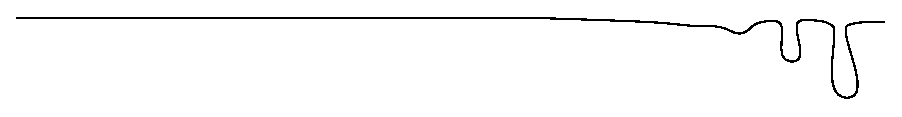
\includegraphics[width=0.6\textwidth]{./plot/sign_line.eps}

\vspace{-1.35cm}
Heidelberg, den 1.April 2015,

%Unterschrift % von der Uni gefordert. ggf anpassen
\end{document}
